\documentclass{beamer}
\usetheme{Madrid}
\usecolortheme{seagull}
\usepackage[utf8]{inputenc}
\usepackage[russian]{babel}
\usepackage{graphicx}

% Информация о презентации
\title[Цифровая обработка звука]{Цифровая обработка звука}
\author[В. Д. Карасев]{Исполнитель: студент группы 221 факультета КНиИТ \\ В. Д. Карасев \\ Руководитель НИР: старший преподаватель М. В. Белоконь}
\institute[Саратов]{Саратовский государственный университет}
\date{Саратов, 2024}

\begin{document}

% Титульный слайд
\begin{frame}
    \titlepage
\end{frame}

% Слайд 2: Удаление артефактов и выравнивание баланса
\begin{frame}{Удаление артефактов и выравнивание баланса}
    \textbf{Удаление шумов и артефактов} Использование инструментов шумоподавления и удаления нежелательных звуков для очистки записи. \\
    \vspace{0.3cm}
    \textbf{Выравнивание баланса:} Регулировка уровней громкости различных элементов аудиозаписи для достижения сбалансированного звучания. \\
    \begin{center}
        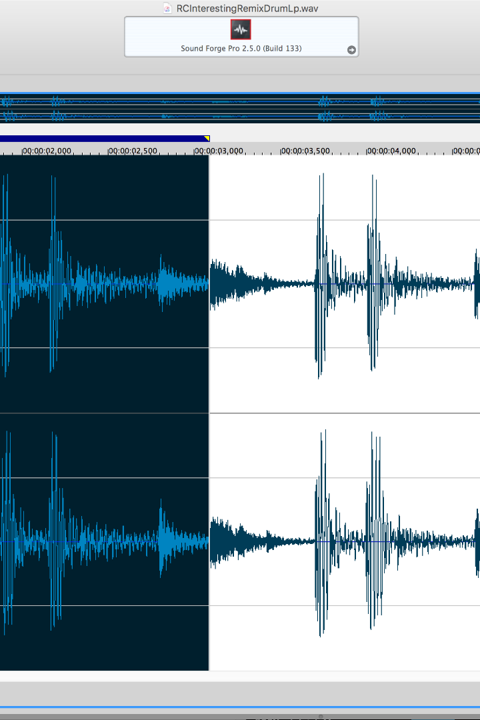
\includegraphics[width=0.6\linewidth]{pic1.png} % Замените на реальное изображение
    \end{center}
\end{frame}

% Слайд 3: Восприятие звука и рекомендации по цифровой обработке
\begin{frame}{Восприятие звука и рекомендации по цифровой обработке}
    \textbf{Восприятие Звука} Понимание того, как человеческое ухо воспринимает различные частоты и динамические диапазоны звука. \\
    \vspace{0.3cm}
    \textbf{Рекомендации по Обработке} Применение знаний о восприятии звука для оптимизации цифровой обработки и достижения желаемого звучания. \\
    \begin{center}
        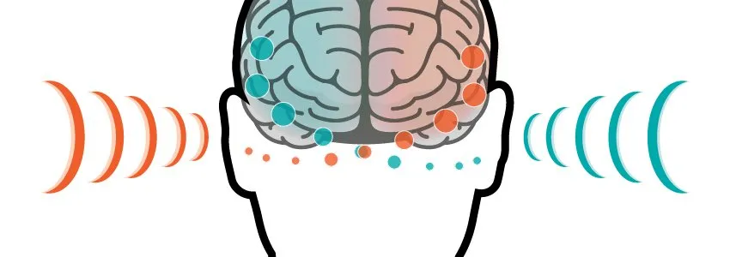
\includegraphics[width=0.6\linewidth]{pic2.png} % Замените на реальное изображение
    \end{center}
\end{frame}

% Слайд 4: Контрастные цвета
\begin{frame}{Характеристики областей звукового диапазона для восприятия}
    \textbf{Низкие Частоты: } Область от 20 Гц до 300 Гц, отвечающая за глубину и фундамент звука. \\
    \vspace{0.3cm}
    \textbf{Средние Частоты: } Область от 300 Гц до 3 кГц, ответственная за разборчивость и присутствие звука. \\
    \vspace{0.3cm}
    \textbf{Высокие Частоты: } Область от 3 кГц до 20 кГц, придающая яркость и детализацию звучанию.
    \begin{center}
        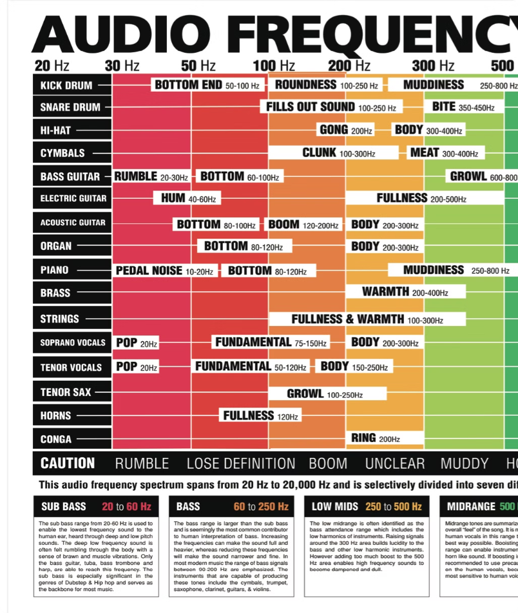
\includegraphics[width=0.6\linewidth]{pic3.png} % Замените на реальное изображение
    \end{center}
\end{frame}

% Слайд 5: Эквалайзер
\begin{frame}{Эквалайзер}
    \textbf{Определение: } Звуковой эквалайзер — это устройство или программный инструмент, который позволяет изменять уровни (громкость) различных частотных диапазонов звука. \\
    \vspace{0.3cm}
    \textbf{Цели: } Эквалайзер используется для коррекции тональности, устранения проблемных частот и улучшения общего звучания. \\
    \vspace{0.3cm}
    \textbf{Принцип Работы: } Эквалайзер разделяет аудиосигнал на отдельные частотные полосы, которыми можно управлять независимо.
    \begin{center}
        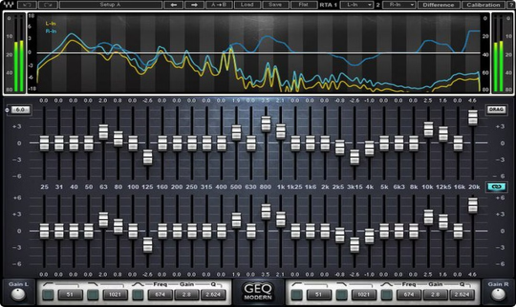
\includegraphics[width=0.6\linewidth]{pic4.png} % Замените на реальное изображение
    \end{center}
\end{frame}

% Слайд 6: Обработка голоса
\begin{frame}{Обработка голоса}
    \textbf{Рекомендации: } Использование эквалайзера для улучшения разборчивости и устранения проблемных частот в голосе. \\
    \vspace{0.3cm}
    \textbf{Диапазоны Голоса: } Мужские голоса обычно находятся в диапазоне 85-180 Гц, женские - 165-255 Гц. \\
    \begin{center}
        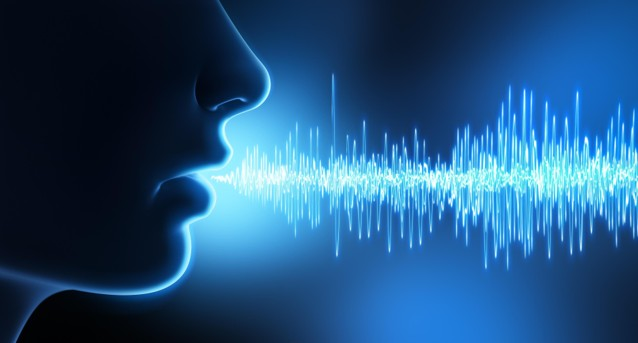
\includegraphics[width=0.6\linewidth]{pic5.jpg} % Замените на реальное изображение
    \end{center}
\end{frame}

% Слайд 7: Сжатие Цифрового Звука
\begin{frame}{Сжатие Цифрового Звука}
	\textbf{Форматы: } Использование форматов сжатия, таких как MP3, WAV и FLAC, для оптимизации размера файлов. \\
	\vspace{0.3cm}
	\textbf{Качество: } Нахождение баланса между качеством звука и размером файла при выборе параметров сжатия. \\
	\vspace{0.3cm}
	\textbf{Битрейт: } Более высокий битрейт обеспечивает лучшее качество, но и больший размер файла.
	\begin{center}
		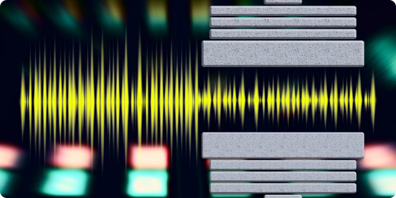
\includegraphics[width=0.6\linewidth]{pic6.png} % Замените на реальное изображение
	\end{center}
\end{frame}

% Слайд 8: Заключение
\begin{frame}{Заключение}
	Цифровая обработка звука - это мощный инструмент для достижения профессионального и полноценного звучания. Применяя техники очистки, обработки голоса и управления частотным диапазоном, мы можем создавать высококачественные аудиозаписи.
	\begin{center}
		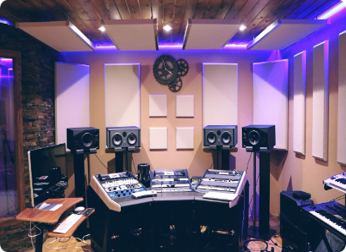
\includegraphics[width=0.6\linewidth]{pic7.png} % Замените на реальное изображение
	\end{center}
\end{frame}

% Слайд 9: Источники
\begin{frame}{Список использованных источников}
    \begin{itemize}
        \item Опенгейм А. В., Шафер Р. В. Цифровая обработка сигналов. Мир, 1979.
        \item Дмитриев В. А. Цифровая обработка сигналов: Учебное пособие. Лаборатория знаний, 2013.
        \item Мюллер М. Fundamentals of Music Processing: Audio, Analysis, Algorithms, Applications. Springer, 2015.
        \item Рэбинар Л., Голд Б. Теория и применение цифровой обработки сигналов. Мир, 1978.
    \end{itemize}
\end{frame}

% Слайд 10: Спасибо за внимание
\begin{frame}
    \centering
    \textbf{\huge Спасибо за внимание!}
\end{frame}

\end{document}
